\documentclass[12pt,a4paper]{article}

% 如果需要中文支持,推荐使用xeCJK + 字体设置
\usepackage{xeCJK}
\setCJKmainfont{SimSun}  % 示例:宋体,可根据系统字体情况更换
\usepackage{amsmath}      % 数学公式(如有需要)
\usepackage{graphicx}     % 插图
\usepackage{geometry}     % 调整页边距
\usepackage{fancyhdr}     % 自定义页眉页脚
\usepackage{indentfirst}  % 中文首行缩进
\usepackage{calc}         % 允许做长度运算(测量文字宽度等)
\usepackage{titlesec}
\usepackage{booktabs} % 解决 \midrule 和 \bottomrule 报错
\usepackage{enumitem} % 支持自定义列表格式
\usepackage{float}
\usepackage{subcaption}
\usepackage{tabularx}

% 设置 \section 级标题为:加粗、大字号(如 \Large)
\titleformat{\section}
	{\bfseries\large}    % 标题自身的格式
	{\thesection}        % 标题编号的显示方式
	{1em}                % 编号与标题文字之间的间距
	{}                   % 在标题文字前后可插入额外代码,此处为空
	
% 设置 \subsection 级标题为:加粗、中等字号(如 \normalsize)
\titleformat{\subsection}
	{\bfseries\normalsize}
	{\thesubsection}
	{1em}
{}

% 页面设置(可根据需要微调)
\geometry{
	left=2cm,
	right=2cm,
	top=1cm,
	bottom=1.5cm
}

% 不需要过大的行距,使用较接近单倍行距的设置
\renewcommand{\baselinestretch}{1}

% 仅在页脚居中显示页码,页眉保持为空
\pagestyle{fancy}
\fancyhf{}  % 清空默认的页眉页脚
\fancyfoot[C]{\thepage}
\renewcommand{\headrulewidth}{0pt}
\renewcommand{\footrulewidth}{0pt}

% 首行缩进2字符(中文习惯)
\setlength{\parindent}{0pt}
\setlength{\leftskip}{2em}

\begin{document}
	%-------------------------------------------------------
	% 1 并排两个minipage:左标题、右校徽
	%   - 0.65\textwidth + 0.35\textwidth = \textwidth
	%   - 如果校徽过大或过小,可改宽度,如 0.25\textwidth、0.3\textwidth 等
	%   - 如果想让标题更大,可将 \Huge 改成 \huge 或 \LARGE
	%-------------------------------------------------------
	\noindent
	\hspace{-2em}
	\begin{minipage}[c]{0.65\textwidth}
		\raggedright
		{\fontsize{40pt}{60pt}\selectfont 物理实验报告}
	\end{minipage}
	\begin{minipage}[c]{0.35\textwidth}
		\raggedleft
		% 强制把校徽拉大到 0.35\textwidth 宽度 (高度自动匹配)
		% 若想指定高度,可用 "height=3cm" 等. 二选一即可.
		
\includegraphics[width=\linewidth, trim={20cm 20cm 20cm 20cm}, clip]{university_logo.png}
	\end{minipage}

	\vspace{-1em}
	

	%下方画两条分割线,并在两线之间写学号、姓名、日期、时间
	
	\hrule
	\vspace{0.4em}
	\noindent
	\begin{tabular}{l l l l}
    学号:\underline{114514} & 姓名:\underline{SUSTech} &
    日期:\underline{2025/03/08} & 时间:\underline{周二下午}
	\end{tabular}
	\vspace{-0em}
	\par
	\hrule

	

	%正文示例

	
	\section{实验名称:测量螺线管的磁场}
	
	\section{实验目的}
	学习测量交变磁场的一种方法,加深理解磁场的一些特性及电磁感应定律。

	\section{实验原理}
	\subsection{有限长载流直螺线管的磁场}
	图1是一个长为2l,匝数为N的单层密绕的直螺线管产生的磁场。当导线中流过电流I时,由毕奥-萨伐尔定律可以计算出在轴线上某一点P的磁感应强度为
		\begin{equation}
		B = \frac{\mu_0 n I}{2} \left\{ \frac{x+l}{\sqrt{R^2+(x+l)^2}} - \frac{x-l}{\sqrt{R^2+(x-l)^2}} \right\}
		\end{equation}
		(1) $\mu_0 = 4\pi\times10^{-7}$ N/A$^2$ \qquad (2) $n = \dfrac{N}{2l}$ 为单位长度上的线圈数\\
		(3) $R$ 为线圈管半径 \qquad (4) $x$ 为 $P$ 点到线圈管中心处的距离\\
		\begin{figure}[htbp]
			\centering
			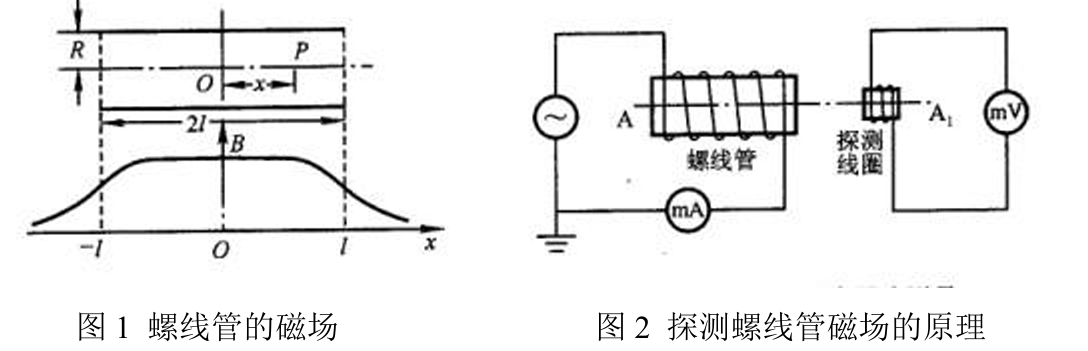
\includegraphics[width=0.40\textwidth]{实验原理.png}
			\caption{实验原理图}
			\label{fig:chart1}
			\end{figure}
		在 SI 单位制中,$B$ 的单位为特斯拉 (T)。图1同时给出 $B$ 随 $x$ 的分布曲线。由曲线显示,在线圈管内部磁场近于均匀,只在端点附近磁感应强度才显著下降。当 $l \gg R$ 时,$B = \mu_0 n I$ 即场点的坐标 $x$ 对内部磁场无影响,而在线圈管两端,
		$B = \frac{1}{2}\mu_0 n I$为内部 $B$ 值的一半。无限长、密绕的直线线圈是实验室中常用的产生均匀磁场的理想装置。
	
	\subsection{探测线圈法测量磁场}
	当低频交流电流通过螺线管产生磁场时,检测线圈中感应出的电压 \(V\) 与磁感应强度 \(B\) 的关系可写为
	\begin{equation}\label{eq:B}
	B = \frac{V}{2\pi^2N_1r_1^2f} \tag{2}
	\end{equation}
	其中,\(N_1\) 为螺线管的匝数,\(r_1\) 为检测线圈半径,\(f\) 为交流电频率。
	
	\section{实验仪器}
	螺线管套件,示波器,信号发生器,电阻,导线若干

	\section{实验内容}
	\subsection{研究螺线管中磁感应强度B与电流I和感生电动势V之间的关系,测量螺线管中的磁感应强度}
	(1) 记录参数:螺线管A的半径R、长度2l、总匝数N,探测线圈A1的半径r1和总匝数N1(参数由实验仪器面板给出)。\\
	(2) 按图2接好线路。需要注意的是,本实验螺线管串联1欧姆的电阻,通过探测电阻两端电压,可以得到输出电流。\\
	(3) A和A1两个中心点的距离代表磁场场点坐标x,其值由装置中的直尺读出。\\
	取x=0(中心位置),低频信号发生器频率分别选取为f=4000Hz、2000Hz、1000Hz,调节信号输出使输出电流从10.0mA至40.0mA,每隔5.0mA记录相应的感生电动势V。\\
	(4)取x=l(管口位置),频率和电流分别取三组数值:f=4000Hz、I=10.0mA;f=2000Hz、I=20.0mA;f=1000Hz、I=40.0mA,测出对应的 V值。从测量结果中可以得出什么结论?\\
	(5)从以上测量数据中取出x=0,f=1000Hz,I=40.0mA和对应的V值,再取x=l,f=1000Hz,I=40.0mA 和对应的V值。分别用公式(1)和(2)计算出B值,并对得出的B值进行比较和讨论。\\

	\subsection{测量直螺线管轴线上的磁场分布}
	(1) 仍按图2接线。取f=2000Hz,输出电流可设定为20.0mA, 当x=0(中心位置)时,记录下此时的V值。\\
	(2) 向外侧移动探测线圈A1,每隔1.0cm记录对应的V,其间注意记下x=l(管口位置)时的V值。测量直至x=21.0cm为止,此时探测线圈中心移出螺线管。\\
	(3) 作出V(x)-x曲线,它是否就是相应的B(x)-x曲线?对曲线进行分析讨论。\\
	(4) 计算\(V_{x=l}/V_{x=0}\) 是否等于 \(\frac{1}{2}\),为什么?

	\section{数据记录}
	根据实验结果记录数据,使用excel整理处理。

	\section{数据处理}
	\subsection{分析讨论V-I曲线}
	根据实验数据,做出散点图并进行线性回归分析,得拟合直线方程及R值。
	\begin{figure}[H]
		\centering
		\begin{subfigure}[b]{0.4\textwidth}
			\centering
			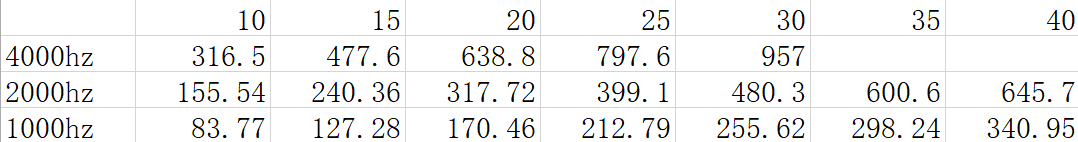
\includegraphics[width=\textwidth]{V-I数据.png}
			\caption{V-I数据}
			\label{fig:chart-amplitude}
		\end{subfigure}
		\hfill
		\begin{subfigure}[b]{0.4\textwidth}
			\centering
			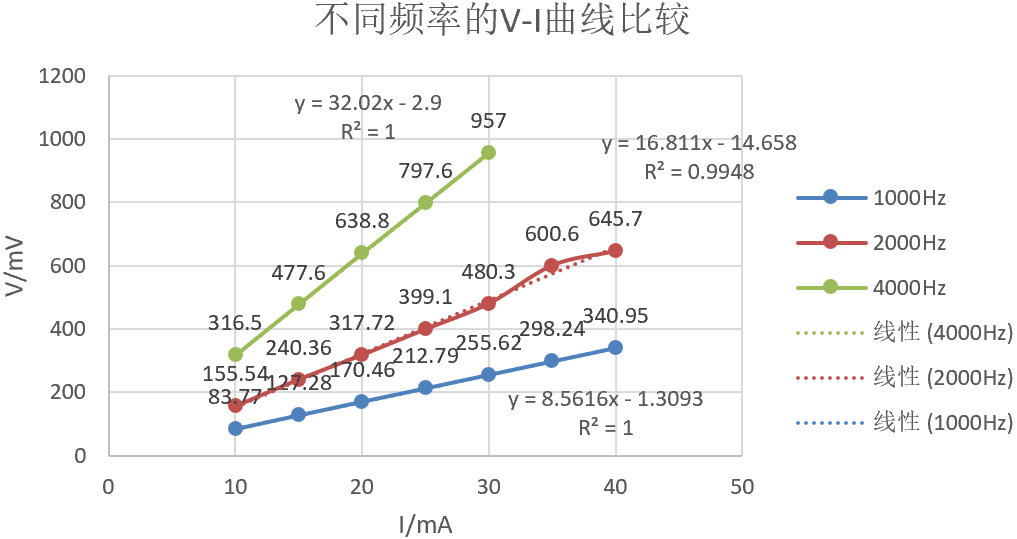
\includegraphics[width=\textwidth]{V-I图.png}
			\caption{V-I图}
			\label{fig:chart-frequency}
		\end{subfigure}
		\caption{V-I曲线}
		\label{fig:chart1}
	\end{figure}	
	直线:当f不变时,由于x=0,故式(1)化为$B=\mu_0 n I$,又有式(2)$B = \frac{V}{2\pi^2N_1r_1^2f}$,得$V=(2\pi^{2}N.r_{1}^{2}fu_{0}n)I$,故V-I呈线性相关\\
	斜率:由V-I图可知:$k_{4000Hz}\approx2k_{2000Hz}\approx4k_{1000Hz}$,刚好与理论公式$V/I=(2\pi^{\prime}Nr_{1}^{2}\mu_{0}n)\cdot f$,斜率与f成正比相符

	\subsection{x=l(管口位置)时,频率和电流得关系}

	\begin{table}[H]
		\footnotesize
		\setlength{\tabcolsep}{3pt}  
		\caption{实验数据(分成两行,每行11组数据)}
		\label{tab:split}
		\begin{tabularx}{\textwidth}{l*{11}{>{\centering\arraybackslash}X}}
		\toprule

		\(x\) (cm) & 0 & 1 & 2 & 3 & 4 & 5 & 6 & 7 & 8 & 9 & 10 \\ 
		\(V\) (mV)   & 320.7 & 320.5 & 320.3 & 320.3 & 320.1 & 319.6 & 318.7 & 318.4 & 318.2 & 317.3 & 316.3 \\ 
		\(B\) (T)    & 0.164678 & 0.164575 & 0.164472 & 0.164369 & 0.164113 & 0.163651 & 0.163394 & 0.162932 & 0.162418 & 0.16211  & 0.161751 \\ 
		\midrule
		\(x\) (cm) & 11 & 12 & 13 & 14 & 15 & 16 & 17 & 18 & 19 & 20 & 21 \\ 
		\(V\) (mV)   & 315.7 & 315   & 312.8 & 309.6 & 302.5 & 281.4 & 238.5 & 181.6 & 126.2 & 74.79 & 29.16 \\ 
		\(B\) (T)    & 0.160621 & 0.158978 & 0.155332 & 0.144497 & 0.122468 & 0.093251 & 0.064803 & 0.038404 & 0.014973 & 0.001119 & 2.18 \\ 
		\bottomrule
		\end{tabularx}
		\end{table}



	同7.1推论公式$V=(2\pi^{\prime}Nr_{1}^{2}\mu_{0}n)\cdot If$同理,得当x=l时,$V = \frac{\pi^2 N_1 r_1^2 f \mu_0 N I}{\sqrt{R^2 + 4l^2}}$\\
	同时由实验数据可看出$f_1 I_1 \approx f_2 I_2 \approx f_2 I_2$,验证了推论公式:fI之积约为定值,故V几乎相等

	\subsection{对计算所得B值比较分析}
	带入要求场景下的实验数据,计算所得制成表格
	\begin{table}[H]
		\centering
		\caption{不同条件下测得的磁场数据}
		\begin{tabular}{|c|c|c|}
		\hline
								  & 公式(1)               & 公式(2)               \\ \hline
		x=0, f=1000\,Hz, I=40.0\,mA & $3.32\times10^{-4}$ & $3.29\times10^{-4}$ \\ \hline
		x=1, f=1000\,Hz, I=40.0\,mA & $1.48\times10^{-4}$ & $1.44\times10^{-4}$ \\ \hline
		\end{tabular}
		\end{table}
	有 $B_1 \approx B'_1$, $B_2 \approx B'_2$,说明测量值与理论值相近;同时有 $B_1 \approx 2B_2$, $B'_1 \approx 2B'_2$,符合 $B_{x=0} = \mu_0 n I = 2\times\frac{1}{2}\mu_0 I = 2B_{x=2}$ 的理论值。
	
	\subsection{V(x)-x曲线与B(x)-x曲线的关系}
	\begin{figure}[H]
		\centering
		\begin{subfigure}[b]{0.4\textwidth}
			\centering
			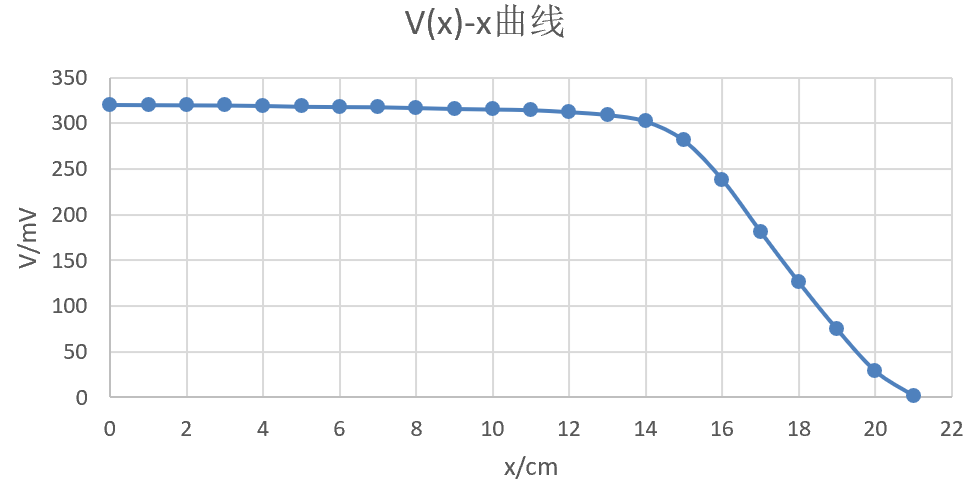
\includegraphics[width=\textwidth]{V-x.png}
			\caption{V-x图}
			\label{fig:chart-amplitude}
		\end{subfigure}
		\hfill
		\begin{subfigure}[b]{0.4\textwidth}
			\centering
			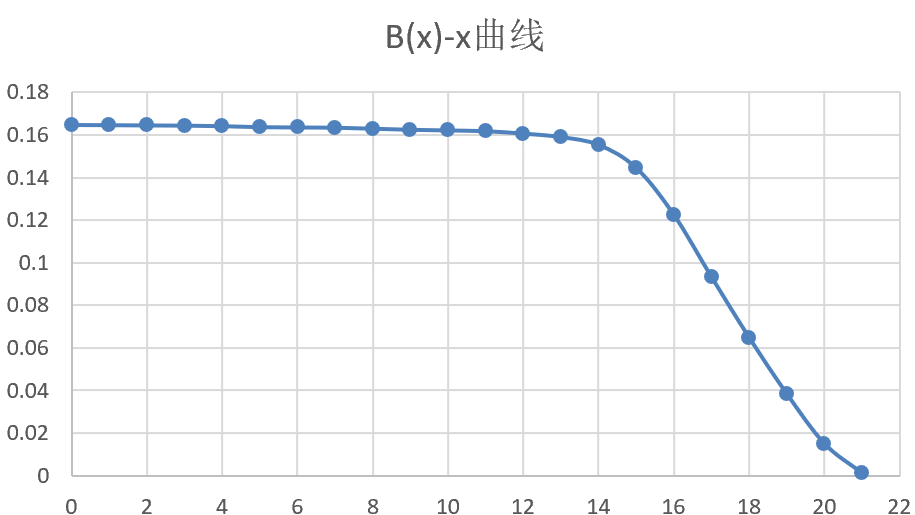
\includegraphics[width=\textwidth]{B-x.png}
			\caption{B-x图}
			\label{fig:chart-frequency}
		\end{subfigure}
		\caption{V(x)-x曲线与B(x)-x曲线对比分析}
		\label{fig:chart1}
	\end{figure}
	做出B(x)-x曲线曲线,与V(x)-x曲线对比,可以发现两者趋势相同,但值不同。\\
	根据$B = \frac{V}{2\pi^2N_1r_1^2f}$,可得$V = B \cdot 2 \pi^2 N_1 r_1^2 f$,实验结果和理论一致。

	\subsection{\( \frac{V_{x=l}}{V_{x=0}} \) 是否等于 \(\frac{1}{2}\)?}
	根据实验数据,其值近似1/2,但由于实际操作中由于漏磁、边缘效应及实验仪器不稳定等一系列原因,造成其值小于1/2。
		\begin{table}[h]
		\centering
		\caption{不同工作条件下的电压数据及其比值}
		\begin{tabular}{cccc}
		\hline
		条件 & \(V_{x=l}\) (mV) & \(V_{x=0}\) (mV) & \(\displaystyle \frac{V_{x=l}}{V_{x=0}}\) \\
		\hline
		\(f=4000\) Hz, \(I=10.0\) mA & 145.4  & 316.5  & 0.46 \\
		\(f=2000\) Hz, \(I=20.0\) mA & 147.76 & 317.72 & 0.465 \\
		\(f=1000\) Hz, \(I=40.0\) mA & 149.36 & 340.95 & 0.438 \\
		\hline
		\end{tabular}
		\end{table}
	
	\subsection{误差分析}

	在实验测量过程中,存在多种可能影响数据精度的误差因素。下面列举了三个主要因素及其分析:
	\begin{enumerate}
    \item \textbf{边缘效应} \\
    理论模型通常假设磁场分布是均匀的,尤其是在螺线管或其他线圈内部采用理想化假设时。然而,在实际情况中,线圈边缘区域的磁场分布往往不均匀,即存在边缘效应。该效应会造成测量点附近的磁通密度与理论预期不同,从而导致电压及其它测量数据产生偏差。边缘效应的影响程度取决于线圈尺寸、匝数以及测量点距离边缘的远近。
    \item \textbf{频率与信号稳定性} \\
    实验中,信号源的频率和电流稳定性对测量结果起着至关重要的作用。如果频率存在较大波动,或信号源在采样过程中不够稳定,会引起瞬时电压值的变化。目前使用的理论公式往往基于稳态信号进行推导,高频下亦可能出现寄生电感、电容等非理想效应,进一步扰乱预期信号。因此,确保信号源和电流源的稳定性是取得准确数据的关键。
    \item \textbf{环境因素} \\
    环境温度、电磁干扰及其他外部因素也会影响实验结果。温度变化可能影响线圈的电阻和电感特性,从而改变通过线圈的电流;同时,外部电磁场的影响可能引入噪声,干扰电压和磁场的稳定测量。为了降低这方面的误差,实验通常需要在温度受控、屏蔽良好的环境中进行,或在数据分析阶段对环境因素造成的误差进行补偿。
	\end{enumerate}


	\section{问题思考}
	为减小测量误差,本实验可从以下几个方面进行改进:
	\begin{enumerate}
  	\item \textbf{仪器精度与校准}  
  	使用高精度的测量仪器,并定期对设备进行校准。增加数据采样次数,通过多次重复测量取平均值,降低系统和随机误差。
  	\item \textbf{环境控制与屏蔽}  
 	建立温度、湿度受控的实验环境,并对实验装置进行电磁屏蔽,减少外部干扰对测量的影响。采用屏蔽室或磁屏蔽设备,可有效降低背景噪声。
  	\item \textbf{实验装置优化}  
  	改进线圈及传感器的设计与制作,尽量减小边缘效应对磁场分布的影响。使用精度更高的元件,并在设计上尽量使磁场分布接近理论模型的理想状态。
  	\item \textbf{信号源稳定性}  
  	为确保信号的频率和幅值稳定,采用高稳定性的波形发生器、电流源和相关控制器,减少因信号波动导致的误差。
  	\item \textbf{同步采样与时序控制}  
  	采用同步采样技术,确保在不同测量位置的数据采集能同步进行,防止因时间延迟或采样误差引起的数据偏差。
	\end{enumerate}

	
	\section{实验结论}
	根据实验过程和实验数据,在数据处理过程进行分析讨论,可以得到部分结论,加深了对磁场的理解。

\end{document}
